% ============================================================
% Capítulo 4 - Metodologia (a plataforma DocFlow e as extensões para a PNIP)
% Base: artigo ICEIS (artigo-iceis-guedes/main.tex), Seção 3 (versão de 16/11/2026).
% ============================================================
\chapter{Metodologia}
\label{cap:metodologia}

Este capítulo descreve a plataforma DocFlow e as extensões feitas nela para a certificação HS da PNIP. O DocFlow transforma em plataforma implementada a arquitetura de assistente para analistas do setor público proposta por \citeonline{Montero2026}, que era conceitual (Seção~\ref{sec:tr-grupo}). Três mudanças de projeto se destacam. Os serviços atrás de um \textit{gateway} de API deram lugar a um monólito modular (Seção~\ref{sec:principios}). O modelo de visão separado deu lugar a LLMs multimodais, que recebem as imagens diretamente (Seção~\ref{sec:execucao}). E a revisão humana, que era uma etapa do fluxo, tornou-se um contrato da API: toda tarefa nasce pendente de revisão, o conteúdo gerado é imutável e toda transição é auditada (Seção~\ref{sec:revisao-humana}). Como o DocFlow foi implementado pelo primeiro autor de \citeonline{Montero2026}, a contribuição deste trabalho está nas extensões descritas nas Seções~\ref{sec:base-conhecimento} e~\ref{sec:execucao} e na sua avaliação na PNIP, relatada no Capítulo~\ref{cap:estudo-caso}.

% ------------------------------------------------------------
\section{Princípios de projeto}
\label{sec:principios}

O DocFlow é um monólito modular escrito em Java~21 com Spring Boot 3.3.5 e Spring AI 1.0, organizado segundo a arquitetura hexagonal (portas e adaptadores). Nessa arquitetura, o domínio e os casos de uso ficam no centro e dependem apenas de interfaces, as portas; o acesso a bancos de dados, a serviços externos e aos provedores de LLM é feito por adaptadores que implementam essas portas. O projeto segue cinco princípios:

\begin{itemize}
	\item \textbf{revisão humana por construção}: a plataforma nunca produz uma decisão final (Seção~\ref{sec:revisao-humana});
	\item \textbf{independência de domínio}: um novo domínio, como a certificação HS, é configuração, e não código;
	\item \textbf{neutralidade de provedor}: OpenAI, Anthropic, Gemini, Ollama e vLLM ficam atrás de uma mesma porta;
	\item \textbf{privacidade desde a concepção}: dados pessoais detectáveis são removidos do texto antes de ele chegar a um LLM;
	\item \textbf{auditabilidade}: execuções, \textit{prompts}, revisões e acessos são registrados.
\end{itemize}

A Figura~\ref{fig:arquitetura} mostra os principais componentes. À esquerda ficam os adaptadores que acionam a plataforma (a API REST, com autenticação e papéis, e um SDK para clientes), usados pelo sistema hospedeiro, como a PNIP; à direita, os adaptadores acionados por ela: extração de texto, OCR e remoção de dados pessoais, armazenamento de objetos (arquivos e fotos), banco vetorial, modelos de \textit{embedding} e provedores de LLM. Como o domínio depende apenas de suas portas, regra verificada por testes de arquitetura com o ArchUnit, trocar o provedor de LLM não altera o domínio. Foi isso que permitiu executar localmente, pelo Ollama, o modelo de \textit{embedding} e os modelos abertos de geração, e acessar os modelos hospedados por suas APIs, sem mudar o restante da plataforma.

\begin{figure}[htb]
	\centering
	\caption{O DocFlow como um hexágono: os adaptadores à esquerda acionam as portas de entrada, e os adaptadores à direita implementam as portas de saída. Todas as dependências apontam para dentro.}
	\label{fig:arquitetura}
	\resizebox{\textwidth}{!}{%
	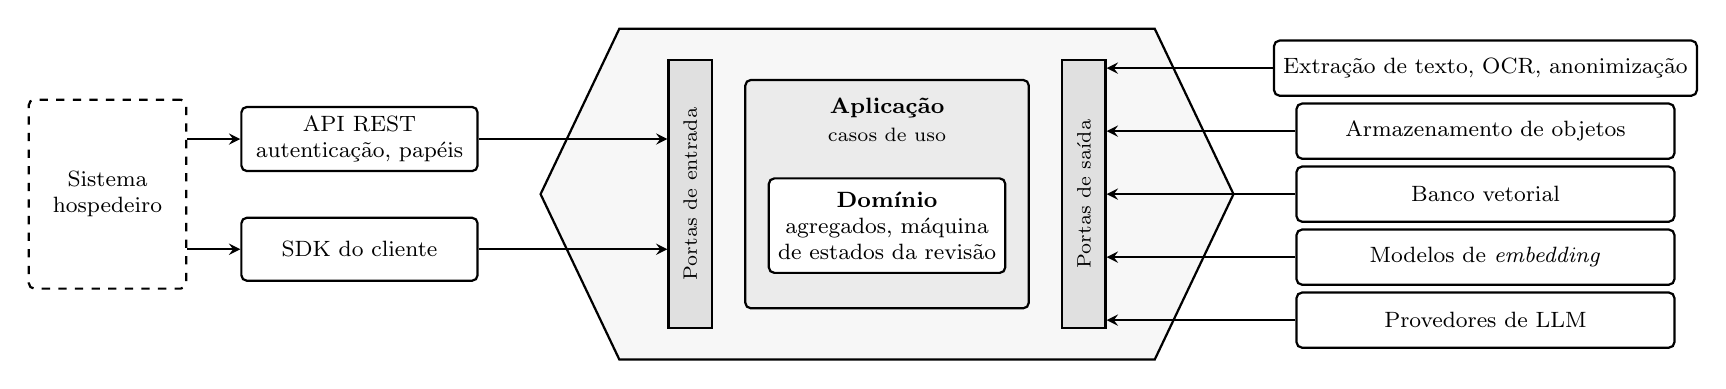
\begin{tikzpicture}[
		font=\footnotesize,
		box/.style={draw, rounded corners=2pt, align=center, minimum height=8mm, fill=white},
		port/.style={draw, minimum width=5.5mm, minimum height=48mm, fill=black!12, font=\scriptsize},
		>=stealth, every path/.style={->, thick}]
		\draw[-, thick, fill=black!3] (-4.4,0) -- (-3.4,2.1) -- (3.4,2.1) -- (4.4,0) -- (3.4,-2.1) -- (-3.4,-2.1) -- cycle;
		\node[box, minimum width=36mm, minimum height=29mm, fill=black!8] (app) at (0,0) {};
		\node[font=\footnotesize\bfseries] at (0,1.1) {Aplicação};
		\node[font=\scriptsize] at (0,0.75) {casos de uso};
		\node[box, minimum width=28mm, minimum height=12mm] at (0,-0.4) {\textbf{Domínio}\\agregados, máquina\\de estados da revisão};
		\node[port, minimum height=34mm] (pin) at (-2.5,0) {\rotatebox{90}{Portas de entrada}};
		\node[port, minimum height=34mm] (pout) at (2.5,0) {\rotatebox{90}{Portas de saída}};
		\node[box, minimum width=30mm] (rest) at (-6.7,0.7) {API REST\\autenticação, papéis};
		\node[box, minimum width=30mm] (sdk) at (-6.7,-0.7) {SDK do cliente};
		\node[box, minimum width=20mm, minimum height=24mm, dashed] (host) at (-9.9,0) {Sistema\\hospedeiro};
		\node[box, minimum width=48mm, minimum height=7mm] (ext) at (7.6,1.6) {Extração de texto, OCR, anonimização};
		\node[box, minimum width=48mm, minimum height=7mm] (obj) at (7.6,0.8) {Armazenamento de objetos};
		\node[box, minimum width=48mm, minimum height=7mm] (vec) at (7.6,0.0) {Banco vetorial};
		\node[box, minimum width=48mm, minimum height=7mm] (emb) at (7.6,-0.8) {Modelos de \textit{embedding}};
		\node[box, minimum width=48mm, minimum height=7mm] (llm) at (7.6,-1.6) {Provedores de LLM};
		\draw (host.east |- rest.west) -- (rest.west);
		\draw (host.east |- sdk.west) -- (sdk.west);
		\draw (rest.east) -- (pin.west |- rest.east);
		\draw (sdk.east) -- (pin.west |- sdk.east);
		\foreach \n in {ext,obj,vec,emb,llm} {\draw (\n.west) -- (pout.east |- \n.west);}
	\end{tikzpicture}}
	\fonte{Adaptada de figura elaborada por Pedro Bilar Montero.}
\end{figure}

Os conceitos centrais da plataforma são quatro. O \textbf{domínio} agrupa a configuração de uma área de aplicação; neste trabalho, \texttt{pnip-hs}. O \textbf{repositório de conhecimento} é um espaço de nomes do índice vetorial, que guarda os documentos indexados para o RAG, aqui as portarias. O \textbf{\textit{workflow}} reúne o modelo de \textit{prompt}, a configuração da recuperação, o provedor de LLM e as opções de recomendação, como os rótulos ``DEFERIR'' e ``INDEFERIR''. E a \textbf{tarefa} é uma execução do \textit{workflow} sobre os documentos de um processo.

% ------------------------------------------------------------
\section{Base de conhecimento e recuperação}
\label{sec:base-conhecimento}

Um repositório de conhecimento guarda documentos indexados para o RAG (Seção~\ref{sec:rag}). A estratégia padrão de segmentação é a recursiva (Seção~\ref{sec:chunking}), com trechos de 512 \textit{tokens} e sobreposição de 100. Os \textit{embeddings} vêm de um modelo local ou hospedado, e os vetores são armazenados no PostgreSQL com o pgvector, sob um índice HNSW com distância de cosseno (Seção~\ref{sec:embedding}). O isolamento entre domínios usa um espaço de nomes composto pelos identificadores do domínio e do repositório, aplicado como filtro em toda consulta.

\subsection{Segmentação por artigo}

Janelas recursivas fariam os trechos de um texto legal começar no meio de um artigo e perder a referência de sua origem. Por isso, foi acrescentada ao DocFlow uma estratégia de segmentação \textit{por artigo}, como em \citeonline{Fiddina2026} e \citeonline{Montero2026}: cada cabeçalho ``Art.~N'' ou ``ANEXO~X'' no início de uma linha abre um trecho, cujo título de seção é o próprio rótulo. Artigos com mais de 2.000 caracteres e textos sem artigos recaem na estratégia recursiva, e os trechos resultantes herdam o rótulo do artigo. Durante o trabalho, um defeito dessa estratégia fez o Art.~17 da Portaria 310/2020 ficar sem trecho próprio, porque havia um espaço antes do rótulo; a expressão regular passou a tolerar espaços iniciais.

\subsection{Recuperação}

Cada trecho é armazenado com o arquivo e o artigo de origem como metadados. A recuperação devolve os $k$ trechos mais similares do espaço de nomes do \textit{workflow} acima de um limiar de similaridade, ambos definidos pelo \textit{workflow}, sem reranqueamento. Na versão original, esses dois parâmetros eram ignorados, e a plataforma sempre recuperava cinco trechos; a correção fez parte das extensões deste trabalho.

Por padrão, a consulta é o texto das instruções da tarefa, igual para todas as tarefas de um \textit{workflow}. Em uma tarefa de análise de processos, isso significa recuperar sempre os mesmos trechos, qualquer que seja o processo (Seção~\ref{sec:rag}). Usar o texto inteiro dos documentos como consulta também não é viável, porque um dossiê de dezenas de milhares de caracteres excede o limite de entrada do modelo de \textit{embedding}. Para esta aplicação, foram acrescentadas as \textbf{consultas por seção}: cada seção dos documentos da tarefa, marcada por um título em Markdown (uma linha iniciada por \texttt{\#\#\#} e seguida do nome da seção), vira uma consulta formada por esse nome e pelos primeiros 2.000 caracteres do texto da seção. Neste trabalho, as seções são as categorias de documento do dossiê, mais o seu cabeçalho. Cada consulta retorna seus $k$ trechos mais similares, e os resultados de todas as consultas são unidos sem repetição, de modo que o contexto depende dos documentos de cada processo. Para usar \textit{embeddings} locais de dimensão menor que a do índice, a plataforma completa os vetores com zeros até a dimensão configurada.

Cada trecho entra no \textit{prompt} precedido de sua origem, no formato \texttt{[Source: arquivo, Art.~N]}, para que se possa pedir ao modelo que o cite. Na versão original, os trechos entravam sem identificação.

% ------------------------------------------------------------
\section{Execução das tarefas}
\label{sec:execucao}

Um cliente cria uma tarefa que referencia um \textit{workflow}, os documentos de entrada e as instruções. Para cada tarefa, a plataforma:

\begin{enumerate}
	\item extrai o texto dos documentos anexados com o Apache Tika, usando o Tesseract para OCR dos documentos digitalizados;
	\item remove do texto endereços de e-mail, números de telefone e de cartão e o CPF (nomes de pessoas não são removidos);
	\item recupera o contexto, quando o \textit{workflow} referencia um repositório de conhecimento;
	\item preenche o modelo de \textit{prompt} com o texto dos documentos, o contexto e as instruções;
	\item encaminha a chamada ao provedor configurado;
	\item extrai uma recomendação procurando os rótulos do \textit{workflow} na resposta e armazena as citações.
\end{enumerate}

A recomendação só é aceita quando exatamente um rótulo aparece. As citações são feitas por trecho quando o RAG está ligado; caso contrário, cada documento anexado é citado como um todo. Cada execução guarda o \textit{prompt} completo, o modelo e a versão do modelo de \textit{prompt}, o que permite auditar e reproduzir o que o modelo recebeu.

\subsection{Entradas de imagem}

A versão original do DocFlow tratava os registros fotográficos apenas como o texto extraído deles por OCR, que em fotos de embarcações é quase sempre vazio ou sem sentido. A plataforma foi estendida para que os documentos de imagem de uma tarefa (PNG e JPEG) cheguem ao modelo como imagens, lidas do armazenamento de objetos e enviadas na ordem em que foram anexadas. O modelo de \textit{prompt} pode informar quantas imagens foram enviadas, e os adaptadores do Ollama, da OpenAI e da Anthropic as enviam junto com a mensagem. Os adaptadores que não aceitam imagens lançam um erro em vez de descartá-las em silêncio. As imagens não passam pela remoção de dados pessoais, que se aplica apenas ao texto.

A ordem das imagens exigiu uma correção adicional: a tabela que liga a tarefa aos seus documentos não guardava a posição de cada documento, e, ao reler a tarefa, a plataforma devolvia as imagens na ordem de seus identificadores. A correção acrescentou uma coluna de posição, preenchida pela ordem de envio (Seção~\ref{sec:dificuldades}).

\subsection{Demais extensões}

Também foram necessárias mudanças nos adaptadores dos provedores. O adaptador do Ollama passou a chamar a API nativa, que permite desligar o modo de raciocínio dos modelos e fixar o tamanho da janela de contexto, algo que a biblioteca Spring AI 1.0 não fazia. O adaptador da OpenAI foi reescrito para enviar as imagens e controlar o esforço de raciocínio, e foi usado também para o Gemini, por meio do \textit{endpoint} compatível com a API da OpenAI. Foi criado um adaptador para a API da Anthropic, com suporte a imagens. Por fim, o tempo limite das chamadas HTTP, de 10 segundos por padrão, foi ampliado, porque a análise de um dossiê com fotos leva minutos em um modelo local.

% ------------------------------------------------------------
\section{Revisão humana como contrato da API}
\label{sec:revisao-humana}

Todo resultado é criado com o estado \textit{pendente de revisão}. O revisor pode aprová-lo, rejeitá-lo (informando o motivo), editá-lo ou pedir que seja gerado de novo. O conteúdo gerado originalmente é imutável: as edições alteram apenas o conteúdo corrente, e cada transição acrescenta um registro de revisão. A aprovação é um estado terminal. Como o contrato está na API, nenhum sistema integrado pode pular a revisão por engano. Na PNIP, isso mantém a decisão com o analista, que é quem responde por ela.

Esse contrato já aparece na integração com a PNIP em desenvolvimento, que não fez parte da configuração avaliada no Capítulo~\ref{cap:estudo-caso}: uma análise assistida verifica 90 regras (25 requisitos da PNIP e 65 itens do programa de autocontrole), o analista aceita ou descarta cada alerta, os itens pendentes bloqueiam o parecer final, e a interface informa que a análise não aprova nem reprova a embarcação.
